\chapter{Dedykowana aplikacja w systemie Android}
\label{ch:aplikacja}
W tym rozdziale pokazana zostanie przykładowa aplikacja która współpracuję z rękawicą-kontrolerem. Aplikacja ta ma za zadanie wyświetlanie aktualnego stanu sensorów rękawicy oraz połączenia, a także prezentowanie tych danych. Pomimo możliwości wykorzystania wielu dostępnych platform do tworzenia animacji oraz środowisk wirtualnych, zdecydowano się na napisanie aplikacji na system Android wykorzystując do tego język Java. Aplikacja ta pozwala na wysoką mobilność, zagłębienie się w tematykę BLE, dzięki zaprogramowaniu własnego połączenia z serwisem udostępnianym przez rękawicę, a także łatwe zaznajomienie się z działaniem rękawicy nawet bez żadnej informacji dotyczącej jej obsługi. Rozdział ten przedstawia interfejs użytkownika, sposób komunikacji z rękawicą-kontrolerem a także opis używanego przez aplikację SDK o nazwie \textit{Google Sceneform}. Dołączony projekt firmy Google pozwala na importowanie modeli dłoni do aplikacji, prezentację ich a także odpowiada za animację na ekranie. W tym rozdziale zostaną pokazane zaimplementowane rozwiązania z którymi mierzą się twórcy kontrolerów, w szczególności przy wykorzystaniu nawigacji inercyjnej.

\section{Interfejs}
\label{sec:interface}
W niniejszej sekcji opisano interfejs wraz z jego elementami oraz ich funkcjonalność w ramach całej aplikacji. Aplikacja składa się z jednej aktywności o nazwie \textit{MainActivity} w ramach której został zaimplementowany układ zakładek, a konkretnie dwóch zakładek - dane oraz animacja. Zakładki te odpowiednio są uzupełnianie przygotowanymi fragmentami poprzez klasę \textit{SectionsPagerAdapter} oraz \textit{ViewPager}.W celu odpowiedniej obsługi fragmentów, aktywność ta musi implementować metody interfejsu \textit{OnFragmentInteractionListener}, które są zadeklarowane w klasach \textit{ModelRenderer} oraz \textit{GloveData}. Klasy te aby spełnić swoją funkcjonalność dziedziczą po klasie \textit{Fragment}~\cite{AndroidDoc}. W ten oto sposób zadeklarowano trzy klasy na podstawie których wyświetlany jest interfejs użytkownika, przedstawiony na rysunku~\ref{fig:ifce}. Metodę \textit{onCreate(Bundle)} przedstawia lsiting~\ref{lst:crt} na którym to widać krok po kroku sposób ładowania fragmentów w aktywności. Dwie ostatnie linie listingu pokazują wywołanie rejestracji odbiornika w celu otrzymywania informacji dotyczącego modułu Bluetooth wbudowanego w urządzenia na którym aplikacja jest uruchomiona. Oprócz wspominanych do tej pory klas, aplikacja korzysta również z dodatkowej klasy o nazwie \textit{VrGlove}, służącej do przechowywania informacji na temat kontrolera. Więcej informacji o tej klasie oraz o odbiorniku modułu Bluetooth zostanie przedstawionych w sekcji~\ref{sec:komunikacja}. 
\begin{lstlisting}[caption={Interfejs użytkownika.},captionpos=b,label={lst:crt},language = Java , frame = trBL , firstnumber = last , escapeinside={(*@}{@*)}]
    @Override
    protected void onCreate(Bundle savedInstanceState) {
        super.onCreate(savedInstanceState);
        setContentView(R.layout.activity_main);
        SectionsPagerAdapter sectionsPagerAdapter = new SectionsPagerAdapter(this, getSupportFragmentManager());
        ViewPager viewPager = findViewById(R.id.view_pager);
        viewPager.setAdapter(sectionsPagerAdapter);
        TabLayout tabs = findViewById(R.id.tabs);
        tabs.setupWithViewPager(viewPager);

        IntentFilter filter = new IntentFilter(BluetoothAdapter.ACTION_STATE_CHANGED);
        registerReceiver(mReceiver, filter);
    }
\end{lstlisting}


\begin{figure}[h]
\centering
	\begin{subfigure}[b]{0.45\textwidth}
	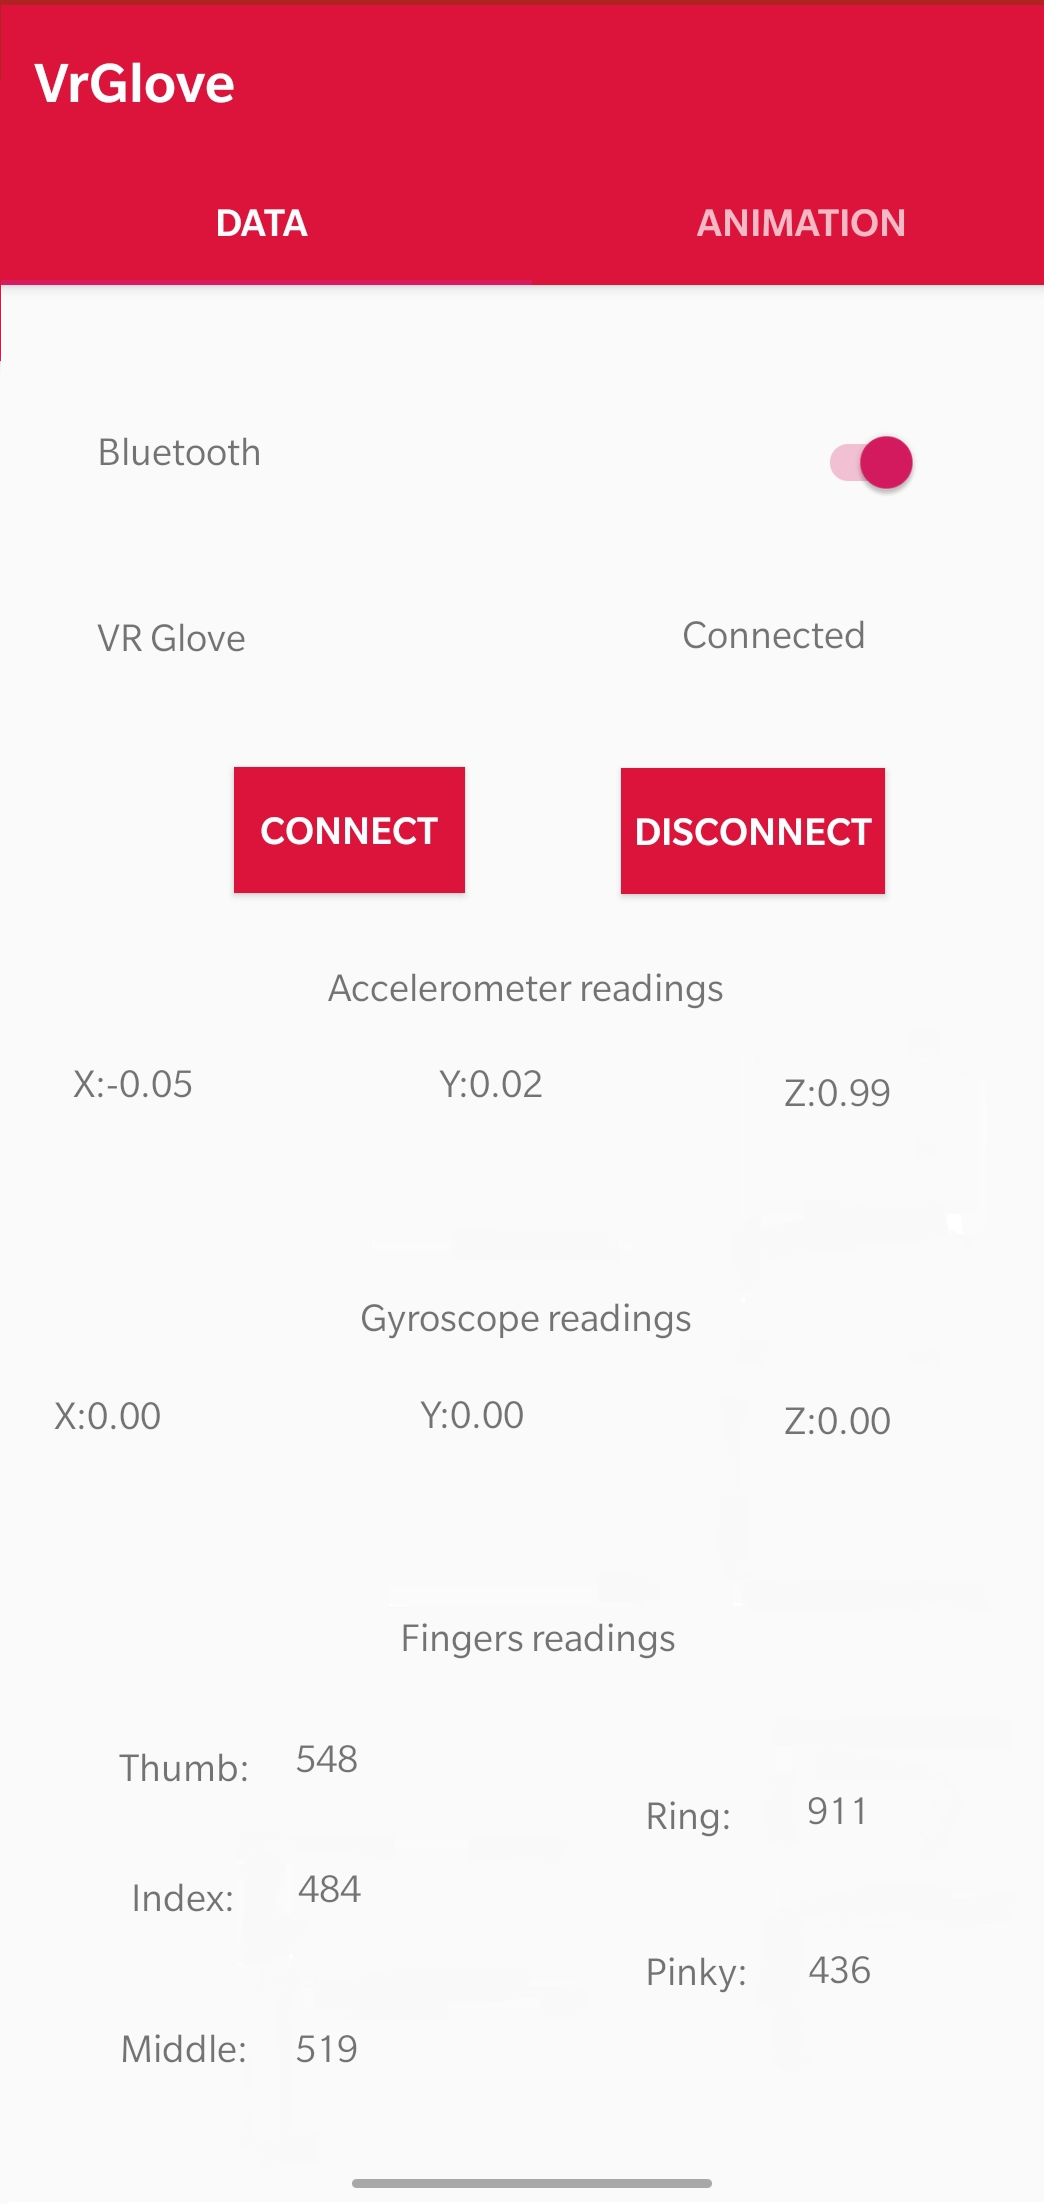
\includegraphics[width=\textwidth]{UI1}
	\caption{Fragment prezentujący dane}
	\label{fig:ifceDane}
	\end{subfigure}
	~
	\begin{subfigure}[b]{0.45\textwidth}
	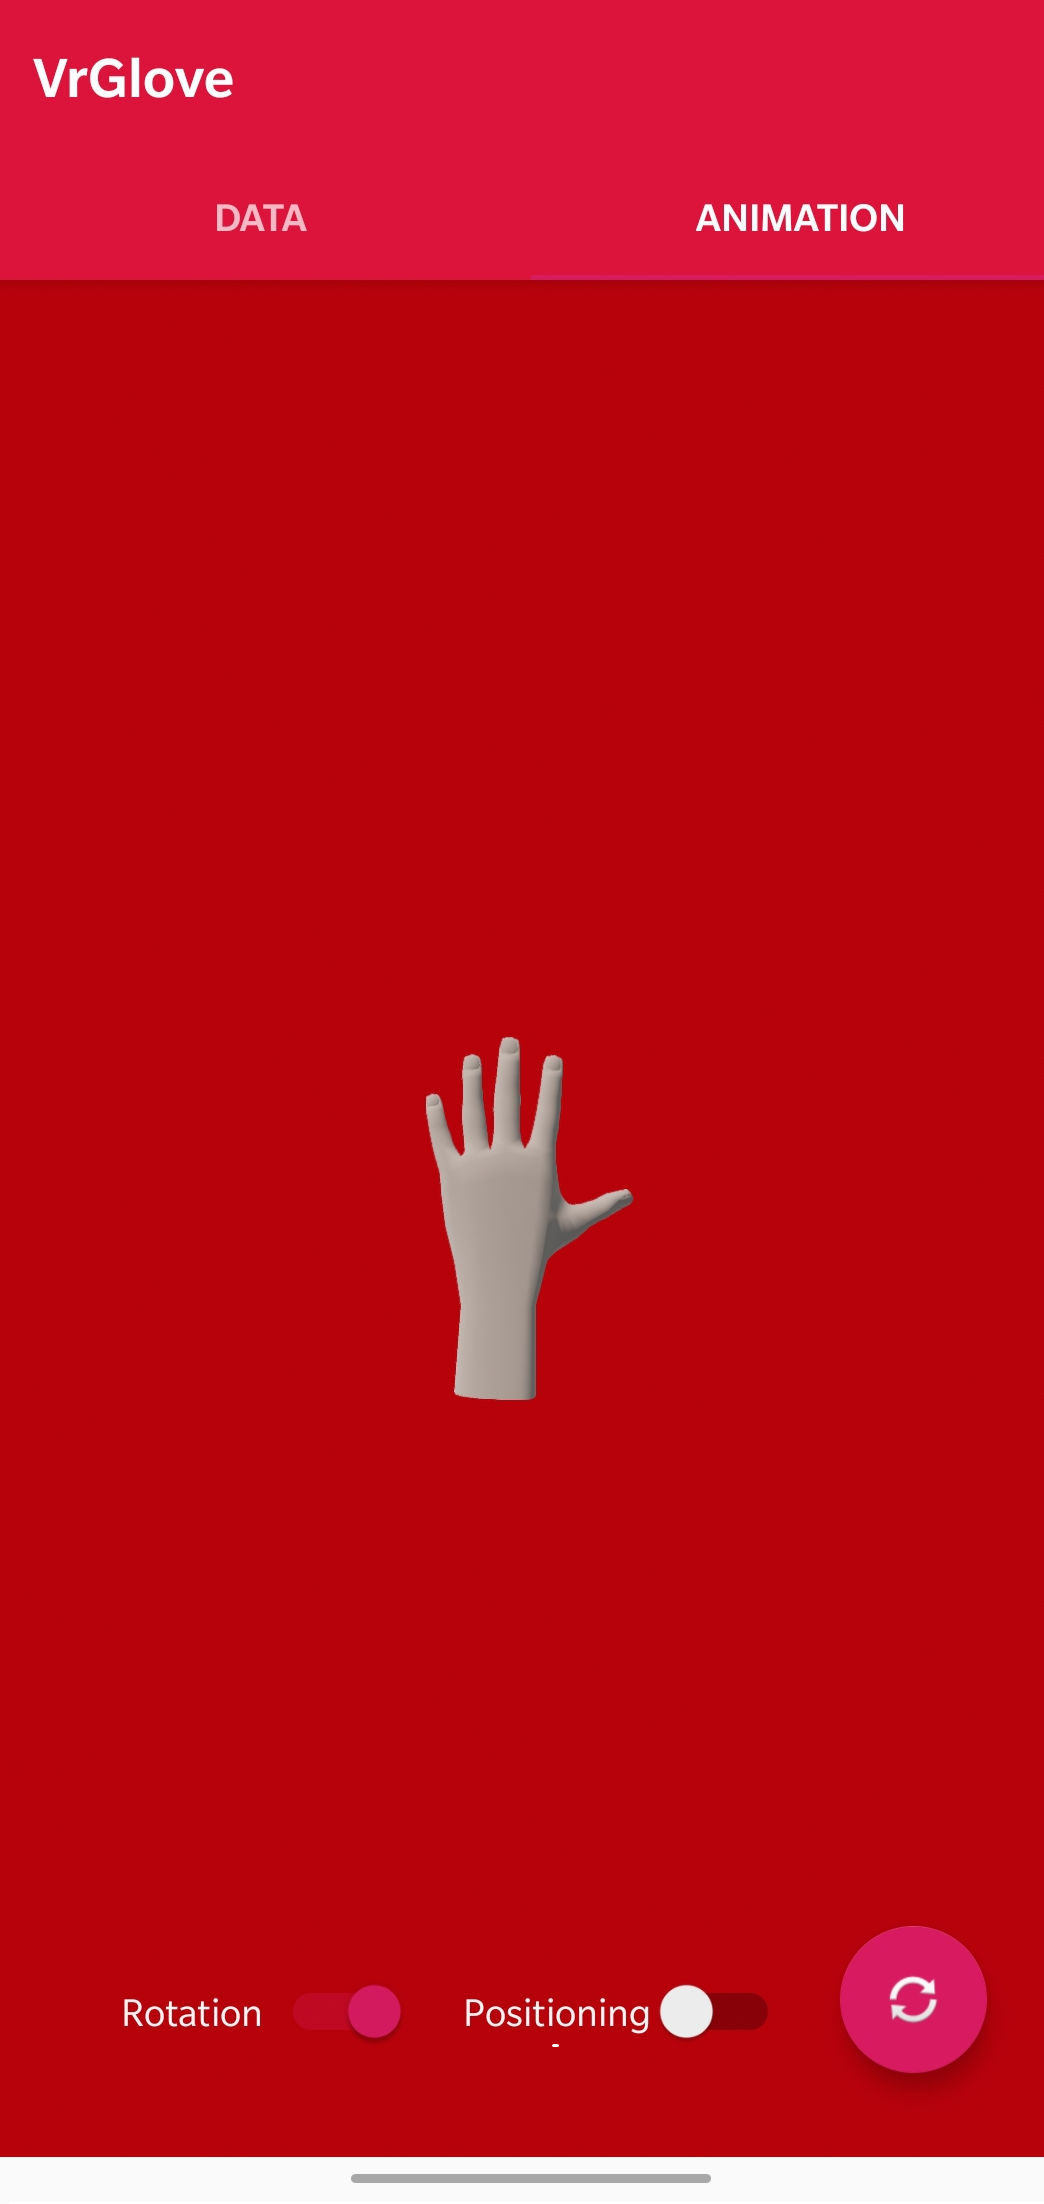
\includegraphics[width=\textwidth]{UI2}
	\caption{Fragment prezentujący animacje}
	\label{fig:ifceAnimacja}
	\end{subfigure}
\caption{Interfejs użytkownika}
\label{fig:ifce}
\end{figure}

Jak widać na~\ref{fig:ifceDane} rozpoczynając od góry widzimy informację dotyczącą obecnego stanu modułu Bluetooth w urządzeniu, wyrażanego poprzez przycisk przełącznika, pozwalający na włączenie/wyłączenie modułu bezpośrednio z poziomu aplikacji. Pod spodem Widnieje informacja o możliwości połączenia/statusie połączenia z kontrolerem opisana etykietą VR Glove. Etykieta ta przyjmuje następujące wartości:
\begin{itemize}
\item Włącz Bluetooth (ang. Turn On Bluetooth)
\item W trakcie włączania (ang. Turning On)
\item W trakcie wyłączania (ang. Turning Off)
\item Gotowy do połączenia (ang. Ready to connect)
\item W trakcie łączenia (ang. Connecting)
\item Połączony (ang. Connected)
\item W trakcie rozłączania (ang. Disconnecting)
\item Rozłączony (ang. Disconnected)
\end{itemize}
\label{itm:stany}
Pierwsze trzy stany możemy osiągnąć poprzez włączanie/wyłączanie modułu Bluetooth w urządzeniu. Stan gotowości do połączenia pokazuję się gdy moduł bluetooth został włączony i jest gotowy do połączenia z kontrolerem. Dwa przyciski znajdujące się poniżej etykiety, odpowiednio \textit{połącz (ang. Connect)} i \textit{rozłącz (ang. Disconnect)} pozwalają na połączenie z rękawicą-kontrolerem. Ostatnie cztery stany obrazują status połączenia z rękawicą, który możemy zmienić korzystając odpowiednio z przycisków. Poniżej znajdują się etykiety dotyczące sensorów kontrolera które są puste gdy aplikacja nie została jeszcze połączona z kontrolerem. Pola ta odpowiednio od góry reprezentują wartości zwracane przez akcelerometr i żyroskop jako wartości X,Y i Z, oraz wartości sensorów znajdujących się na palcach, z każdym sensorem mającym własną etykietę. Drugą częścią interfejsu prezentuje~\ref{fig:ifceAnimacja}, na której to widoczna jest lewa dłoń, znajdujące się na środku ekranu. Pozycja ta jest przyjmowana zanim kontroler zostanie podłączony. W dolnej części ekranu widzimy dwa przyciski przełączniki, służące do regulowania modelu, pozwalając decydować nam które elementy mają być brane pod uwagę podczas generowania animacji. Od lewej odpowiednio możliwe jest do zmiany branie pod uwagę orientacji kontrolera przy generowaniu modelu, następnie jego pozycji względem pozycji kalibracyjnej, oraz ostatni element tego interfejsu czyli FAB(z ang. Floating Action Button) - służący do ponownej kalibracji dłoni. Kalibracja ta jest również wywoływana przy każdej zmianie decyzji dotyczącej generowania rotacji bądź położenia. Pozycją kalibracyjną jest pozycja w której lewa dłoń na której znajduje się rękawica-kontroler, wraz ze wszystkimi palcami znajduję się w pozycji wyprostowanej, a kciuk wskazuje ciało użytkownika. Interfejs ten pozwala na szybkie połączenie się z kontrolerem a gdy tylko pierwsze dane zostaną przesłane do aplikacji, natychmiastowo obserwujemy pracę kontrolera na ekranie smart-fona. Warto zauważyć że po włączeniu aplikacji przełącznik orientacji jest włączony natomiast pozycjonowanie dłoni na ekranie wyłączone, w związku z czym animacja wyświetla się na środku ekranu. Do tej pory opisano wygląd i informacje elementów znajdujących się na ekranie, dalsza część tego rozdziału pokaże w jaki sposób wspomniane elementy działają od strony kodu źródłowego.

\section{Komunikacja}
\label{sec:komunikacja}
Opis interfejsu aplikacji pokazuje elementy które są wymagane oraz zaprogramowane w aplikacji. Pokazuje jakie dane są używana oraz w jakim celu wykorzystywane. Żeby jednak skorzystać z tych danych najpierw aplikacja musi zostać połączona z kontrolerem. W sekcji~\ref{subsec:arduino} powiedziano o wykorzystywaniu w tym celu połączenia BLE a o tym jak to jest obsługiwane przez prezentowaną aplikacje zostanie pokazane w części~\ref{subsec:ble}. Aby rozpocząć pracę z BLE przede wszystkim należy się upewnić że moduł Bluetooth w urządzeniu jest dostępny oraz włączony. W celu sprawdzenia dostępności modułu bluetooth w urządzeniu wykorzystywany jest plik \textit{AndroidManifest.xml}, w którym to zdefiniowano dostęp. Wszystkie wymagane pozwolenia pokazuje listing~\ref{lst:pozwolenia}.
	\begin{lstlisting}[caption={Wymagane pozwolenia dla aplikacji.},captionpos=b,label={lst:pozwolenia},language = Java , frame = trBL , firstnumber = last , escapeinside={(*@}{@*)}]
    <uses-permission android:name="android.permission.BLUETOOTH" />
    <uses-permission android:name="android.permission.BLUETOOTH_ADMIN" />
    <uses-permission android:name="android.permission.READ_EXTERNAL_STORAGE" />
    <uses-permission android:name="android.permission.CAMERA" />
\end{lstlisting}
Mając wymagany dostęp możemy sterować sensorem poprzez przycisk przełącznika. W kodzie programu wystarczy uzyskać do niego dostęp używając metody \textit{findViewById(int)} a następnie ustawić nasłuchiwacza kliknięć. Przyciski \textit{Połącz} oraz \textit{Rozłącz} są zdefiniowane w ten sam sposób. Aby wprowadzić zmiany w Bluetooth należy użyć klasy \textit{BluetoothAdapter}. Po pobraniu domyślnego adaptera jesteśmy w stanie określić jego stan. używając metod \textit{enable()} oraz \textit{disable()}. Sposób obsługi adaptera jest pokazany na listingu~\ref{lst:switchBT}. Zmiana ta wywołuję funkcję znajdującą się w klasie \textit{MainActivity} która reaguje na zmiany adaptera oraz ustawia jeden z pierwszych czterech statusów z listy~\ref{itm:stany} dla pola definiującego obecny stan połączenia. Skrócony listing~\ref{lst:status} pokazuje wywołanie tej funkcji dla przykładowego stanu adaptera. Ostatnie cztery stany wypunktowane w~\ref{itm:stany} pochodzą ze zmiany połączenia wywoływane poprzez wspomniane przyciski \textit{Połącz} oraz \textit{Rozłącz} które zostoną opisane w sekcji~\ref{subsec:ble}.
	\begin{lstlisting}[caption={Obsługa wbudowanego modułu Bluetooth.},captionpos=b,label={lst:switchBT},language = Java , frame = trBL , firstnumber = last , escapeinside={(*@}{@*)}]
switch (v.getId()){
            case R.id.switchBT:
            	Switch switchBT = v.findViewById(R.id.switchBT);
        		BluetoothAdapter mBluetoothAdapter = BluetoothAdapter.getDefaultAdapter();
                if (switchBT.isChecked()){
                    if (!mBluetoothAdapter.isEnabled()) {
                        mBluetoothAdapter.enable();
                    }
                }else{
                    if (mBluetoothAdapter.isEnabled()) {
                        mBluetoothAdapter.disable();
                    }
                }
                break;
                [...]
}
\end{lstlisting}
\begin{lstlisting}[caption={Zmiana statusu na podstawie adaptera bluetooth.},captionpos=b,label={lst:status},language = Java , frame = trBL , firstnumber = last , escapeinside={(*@}{@*)}]
private final BroadcastReceiver mReceiver = new BroadcastReceiver() {
        @Override
        public void onReceive(Context context, Intent intent) {
            final String action = intent.getAction();
            Switch tbBT= findViewById(R.id.switchBT);
            TextView tvStatus = findViewById(R.id.textView_vrGlove_status);
            if (action.equals(BluetoothAdapter.ACTION_STATE_CHANGED)) {
                final int state = intent.getIntExtra(BluetoothAdapter.EXTRA_STATE,
                        BluetoothAdapter.ERROR);
                switch (state) {
                    case BluetoothAdapter.STATE_OFF:
                        tbBT.setChecked(false);
                        tvStatus.setText("Turn on bluetooth");
                        break;
                    [...]
}                    
\end{lstlisting}

	\subsection{Obsługa połączenia Bluetooth Low Energy}
	\label{subsec:ble}
	Gdy poznano stan modułu Bluetooth, bez przeszkód można nawiązać połączenie. w tym celu wykorzystano przyciski sterujące połączeniem. Do przechowywania danych o połączeniu wykorzystywana jest klasa \textit{VrGlove}, w której zdefiniowano statyczne zmienne klasy \textit{BluetoothDevice} pozwalające na wybranie odpowiedniego urządzenia z puli dostępnych urządzeń w pobliży poprzez jego adres oraz \textit{BluetoothGatt} odpowiedzialnej za obsługę \textit{GATT} (z ang. Generic Attribute Profile) w androidzie. Listę dostępnych serwisów otrzymano deklarując zmienną implementującą listę klasy  \textit{BluetoothGattService}. W ten sposób w dowolnym miejscu programu można odwołać się do klasy kontrolera, sprawdzając jego stan a także uzyskać dane o jego udostępnionych serwisach. W ten oto sposób na listingu~\ref{lst:disconnect} pokazano dostęp do klasy rękawicy z nasłuchiwacza przycisku \textit{Rozłącz}. Fragment ten sprawdza czy istnieje aktualnie połączony serwis \textit{GATT} oraz czy jest on w stanie \textit{Połączony} wyrażony jako typ \textit{int} - 2. To właśnie na podstawie tego statusu są określane ostatnie cztery stany połączenia z rękawicą z listy~\ref{itm:stany}. Sposób zmiany statusu są bardzo zbliżone do listingu~\ref{lst:status}, różnica polega na wywołaniu odbiornika zmiany statusu połączenia z klasy \textit{BluetoothGattCallback} w przeciwieństwie do \textit{BroadcastReceiver} oraz zostaje wywołana metoda \textit{onConnectionStateChange} zamiast metody \textit{onReceive}. Jeżeli powyższe warunki są spełnione \textit{GATT} zostaje rozłączony~\cite{AndroidDoc}. 
\begin{lstlisting}[caption={Obsługa przycisku rozłącz.},captionpos=b,label={lst:disconnect},language = Java , frame = trBL , firstnumber = last , escapeinside={(*@}{@*)}]
case R.id.buttonDisconnect:
                if(VrGlove.getGatt() != null && VrGlove.getGattState() == 2 ){
                    VrGlove.getGatt().disconnect();
                }
                break;                    
\end{lstlisting}	
Ostatnia część którą opisano jest zarazem najważniejszą. Mowa o obsłudze przycisku \textit{Połącz}. Tak jak w przypadku przycisky \textit{Rozłącz}, najpierw sprawdzany jest status urządzenia, czyli czy adapter jest włączony oraz w przeciwieństwie do sprawdzania czy nasz serwis \textit{GATT} jest połączony, kod przycisku wykona się tylko wtedy gdy nie jest aktualnie nawiązane połączenie. Gdy warunki te są spełnione, zostaje pobrany adapter bluetooth oraz zostaje podjęta próba połączenia z urządzeniem przy użyciu klasy \textit{BluetoothDevice}, która otrzymuje zwracaną wartość metody \textit{getRemoteDevice(String)} wywołaną na adapterze bluetooth. W naszym przypadku jako parametr typu \textit{String}, zostaje podany adres \textit{D0:6B:F2:A7:95:03}, który jest adresem rękawicy-kontrolera z którym zostanie podjęta próba połączenia. Następnie zostaje stworzona nowa instancja klasy \textit{VrGlove}, której zostaje przekazana w parametrach wartość zmiennej typu \textit{BluetoothDevice} oraz aktualny widok na którym pracuje fragment. Posiadając te informacje rozpoczyna się kluczowy etap połączenia, mianowicie zostaje zainicjalizowana zmienna klasy \textit{BluetoothLeScanner}, poprzez wywołanie metody \textit{getBluetoothLeScanner()} na adapterze urządzenia. Metoda ta pozwala na wyszukiwanie urządzeń BLE znajdujących się w pobliżu, poprzez wywołanie metody \textit{startScan(ScanCallback)}, gdzie jako parametr zostaje podany stworzony skaner, oczekujący na pojawienie się urządzenia z wcześniej podanym adresem. Bardzo ważnym elementem jest zatrzymanie skanera gdy zostaje odnalezione urządzenie - co można osiągnąć poprzez wywołanie metody \textit{stopScan(ScanCallback)}. W ten oto sposób nawiązano połączenie pomiędzy urządzeniami a rezultat tego połączenie zostaje zapisany w postaci ustawienia serwisu \textit{GATT} w klasie \textit{VrGlove}. Opisane powyżej czynności są przedstawione na listingu~\ref{lst:connect}~\cite{AndroidDoc}. W ten oto sposób możemy kontrolować połączenie z kontrolerem z dedykowanej aplikacji. Ostatnim elementem poprawnego funkcjonowania jest przekazywanie danych w czasie rzeczywistym pomiędzy odbiornikiem a nadajnikiem, co zostanie pokazane w sekcji~\ref{subsec:dane}.
\begin{lstlisting}[caption={Kluczowe elementy przycisku \textit{Połącz} pozwalającego na połączenie z kontrolerem.},captionpos=b,label={lst:connect},language = Java , frame = trBL , firstnumber = last , escapeinside={(*@}{@*)}]
final BluetoothManager bluetoothManager =
                            (BluetoothManager) getActivity().getSystemService(Context.BLUETOOTH_SERVICE);
mBluetoothAdapter = bluetoothManager.getAdapter();
[...]
BluetoothDevice device = mBluetoothAdapter.getRemoteDevice("D0:6B:F2:A7:95:03");
new VrGlove(device,vw);                    
[...]
BluetoothLeScanner scanner = mBluetoothAdapter.getBluetoothLeScanner();
scanner.startScan(scanCallback);
[...]
scanner.stopScan(scanCallback);
gatt = VrGlove.getDevice().connectGatt(getActivity(),false,bluetoothGattCallback, TRANSPORT_LE);
VrGlove.setGatt(gatt);                                                           
\end{lstlisting} 

	\subsection{Pobieranie danych}
	\label{subsec:dane}
	Mając do dyspozycji informacja pozyskane w trakcie połączenia, które są przechowywane jako zmienne statyczne w klasie rękawicy, jesteśmy w stanie pozyskać dane które opisano w rozdziale~\ref{ch:rekawica}. W tym celu, po stronie aplikacji należy sprawdzić czy aktualnie jest nawiązane połączenie, co jak już zostało powiedziane oznacza serwis \textit{GATT} w stanie wyrażanym jako \textit{int = 2}.  Gdy potwierdzono połączenie, z klasy \textit{BluetoothGatt} zostaje wywołana metoda \textit{discoverServices()}, która jest wywoływana dopóki nie zostaną wykryte serwisy. Gdy tak się stanie, rezultat odnalezionych serwisów uzyskiwany jest poprzez metodę serwisu \textit{GATT} \textit{getServices()}. Mając dostęp do serwisów - w opisywanym przypadku wiemy z rozdziału dotyczącego rękawicy-kontrolera że jest to tylko jeden serwis, możemy pobrać cechy używając metody \textit{getCharacteristic(UUID)}, które ten serwis posiada. Cechy te zostały pokazane na listingu~\ref{lst:deklaracje}, oraz zostały przypisane im skrócone UUID wyrażone jako \textit{int} od $0x2101$ do $0x2103$, odpowiednio jako dane akcelerometru, żyroskopu oraz sensorów umiejscowionych na palcach. Implementacje algorytmu z typu \textit{int} do UUID pokazuje metoda \textit{convertFromInteger(int i)} na listingu~\ref{lst:UUID}~\cite{UUID}. 
	\begin{lstlisting}[caption={Zamiana zmiennej int na UUID.},captionpos=b,label={lst:UUID},language = Java , frame = trBL , firstnumber = last , escapeinside={(*@}{@*)}]
	private UUID convertFromInteger(int i) {
        final long MSB = 0x0000000000001000L;
        final long LSB = 0x800000805f9b34fbL;
        long value = i & 0xFFFFFFFF;
        return new UUID (MSB | (value << 32), LSB);
    }                                                       
\end{lstlisting}
Dla każdej cechy zostaje wywołana metoda \textit{readCharacteristic(BluetoothGattCharacteristic)}, która po sprawdzeniu warunków które są wymagane od każdej z cech dla prezentowanej aplikacji ustawia te cechy w trybie powiadomień - etap ten prezentuje listing~\ref{lst:notify}. Tryb powiadomień dla cechy oznacza że dane zostaną pobrane za każdym razem gdy zajdzie w nich jakaś zmiana. Ostatnią częścią jest pobranie deskryptora danej cechy. W ten sposób oprócz nawiązanego połączenia uzyskano dostęp do serwisów oraz cech reprezentowanych przez urządzenie z którym się połączono. Etap ten zaprezentowano na wycinku kodu~\ref{lst:characteristics}.

\begin{lstlisting}[caption={Uzyskanie dostępu do cech serwisu.},captionpos=b,label={lst:characteristics},language = Java , frame = trBL , firstnumber = last , escapeinside={(*@}{@*)}]     
if(VrGlove.getGattState() == 2){
	VrGlove.getGatt().discoverServices();                                                   
	[...]
	VrGlove.setServices(VrGlove.getGatt().getServices());
	for (int i = 0x2101;i<0x2104;i++){
    	mCharacteristic = VrGlove.getServices().get(2).getCharacteristic(convertFromInteger(i));
        readCharacteristic((mCharacteristic));
        BluetoothGattDescriptor descriptor = mCharacteristic.getDescriptor(convertFromInteger(0x2902)); 
        [...]
        VrGlove.getGatt().writeDescriptor(descriptor);
}
\end{lstlisting}

\begin{lstlisting}[caption={Ustawienie cechy w trybie powiadomień.},captionpos=b,label={lst:notify},language = Java , frame = trBL , firstnumber = last , escapeinside={(*@}{@*)}]     
private boolean readCharacteristic(final BluetoothGattCharacteristic characteristic) {  
        if(VrGlove.getGatt() == null) {
            Log.e(TAG, "ERROR: Gatt is 'null', ignoring read request");
            return false;
        }
        if(characteristic == null) {
            Log.e(TAG, "ERROR: Characteristic is 'null', ignoring read request");
            return false;
        }
        if((characteristic.getProperties() & PROPERTY_READ) == 0 ) {
            Log.e(TAG, "ERROR: Characteristic cannot be read");
            return false;
        }
        VrGlove.getGatt().setCharacteristicNotification(characteristic, true);
        return true;
    }                                                      
\end{lstlisting}

Ważnym elementem tego procesu jest odczytywanie cech pojedynczo, z racji tego że serwis \textit{GATT} obsługuję połączenie tylko z jedną cechą jednocześnie, co oznacza że gdyby spróbowano pobrać następną cechę, podczas gdy połączenie nie zostało zakończone z poprzednią cechą - połączenie to zostanie nadpisane. Obsługę połączenia z cechą zapewnia nadpisanie metody \textit{onCharacteristicChange(BluetoothGatt, BluetoothGattCharacteristic)} wywoływaną  z klasy \textit{BluetoothGattCallback}. Kod został napisany właśnie w tej metodzie ze względu na tryb w jaki cechy zostały ustawione, czyli tryb powiadomień. Dzięki temu funkcja ta zostaje wywołana za każdym razem gdy obserwowane cechy zostaną w jakiś sposób zmienione. W zależności od rozpoznanej cechy, wywoływana jest metoda zmieniające aktualny zestaw danych w klasie kontrolera, co pokazuje listing~\ref{lst:findChar}. Następnie funkcje klasy \textit{VrGlove} przypisują zmiennym odpowiadającym sensorom nowe dane oraz dokonują ich konwersji z tablicy typu \textit{byte} do typu \textit{float}. Dane te po obróbce są przypisywane odpowiednim polom w interfejsie użytkownika. Pobieranie danych polega na wycinaniu z tablicy informacji kolejnych 4 bajtów, co jest równoznaczne jednej zmiennej typu \textit{float}. Ważne dla konwersji jest również sposób w jaki dane zostają zamienione - w tym przypadku używana jest notacja \textit{LITTLE\_ENDIAN}. Wykonane kroki pokazuje listing~\ref{lst:setChar} dla odczytu pierwszej wartości z tablicy danych żyroskopu. Proces ten należy wykonać dla wszystkich wartości w danej cesze oraz odpowiednio dla każdej z pobieranych cech~\cite{AndroidDoc}.
\begin{lstlisting}[caption={Odczytywanie danych cechy.},captionpos=b,label={lst:findChar},language = Java , frame = trBL , firstnumber = last , escapeinside={(*@}{@*)}]     
 if(characteristic.getUuid().equals(convertFromInteger(0x2101))){
	VrGlove.setAccReadings(value);
}else if (characteristic.getUuid().equals(convertFromInteger(0x2102))){
	VrGlove.setGyroReadings(value);
}else if(characteristic.getUuid().equals(convertFromInteger(0x2103))){
	VrGlove.setFingersReadings(value);
}else{
	Toast.makeText(getActivity(),"Unknown characteristic",Toast.LENGTH_SHORT);
}                                                   
\end{lstlisting}

\begin{lstlisting}[caption={Przypisywanie danych pozyskanych z cech, do zmiennych w aplikacji.},captionpos=b,label={lst:setChar},language = Java , frame = trBL , firstnumber = last , escapeinside={(*@}{@*)}]     
     static void setGyroReadings(byte[] gyroReadings) {
        VrGlove.gyroReadings = gyroReadings;
        getGyroReadings();
    }      
    
     private static void getGyroReadings() {
        TextView x = vw.findViewById(R.id.textView_gyr_X);
        Float[] data = new Float[3];
        
        float f = ByteBuffer.wrap(gyroReadings,0,4).order(ByteOrder.LITTLE_ENDIAN).getFloat();
        data[0] = f;
        x.setText(String.format("X:%.2f",f));
      	[...]

        dataSet.put("Gyro",data);
        setmIsStateChanged(true);
    }                                      
\end{lstlisting}

W tej sekcji został pokazany sposób połączenia aplikacji z kontrolerem, oraz sposób w jaki po ustanowieniu połączenia dane zostają przekazane i obrabiane. W ten sposób fragment \textit{GloveData}, odpowiedzialny za prezentację interfejsu pokazanego na rysunku~\ref{fig:ifceDane} kończy swoje działanie. Na podstawie tych danych fragment \textit{ModelRenderer} jest w stanie wygenerować drugą część interfejsu która zostanie teraz opisana.

\section{Google Sceneform SDK}
\label{sec:sceneform}
Jak widać na zdjęciu interfejsu~\ref{fig:ifceAnimacja}, drugi fragment prezentuje dłoń, której pozycja, orientacja oraz kształt zmienia się w czasie rzeczywistym. Aby to osiągnąć zdecydowano się na wybór SDK udostępnionego od \textit{Google}, służącego do renderowania realistycznych scen w aplikacjach na androida. Pomimo oryginalnego zastosowania służącego do budowania aplikacji AR (z ang. Augmented Reality), zestaw narzędzi został rozbudowany do obsługi aplikacji spoza tej dziedziny. W ten oto sposób, bez znajomości OpenGl otrzymano dostęp między innymi do narzędzi, obsługujących scenę na której renderowane są obrazy, a także wtyczki do Android Studio, pozwalającej na importowanie modeli 3D do aplikacji w prosty sposób. Wtyczkę dodano do środowiska programistycznego poprzez wyszukanie w menu \textit{Wtyczki}, wtyczki o nazwie \textit{Google Sceneform Tools (Beta)}. W ten oto sposób po kliknięciu prawym przyciskiem myszy na model znajdujący się w drzewie projektu, pojawia się opcja \textit{zaimportuj model}, tworząca dwa pliki na podstawie których \textit{Sceneform} generuje model na ekranie: \textit{.sfa} oraz \textit{.sfb}. Gdy zainstalowano wtyczkę, należy pobrać z oficjalnego linku do strony projektu Github foldery zawierające SDK. Foldery te należy dodać do projektu, które od teraz są jego częścią. Szczegółowy opis jak przeprowadzić ten proces znajduję się w dokumentacji SDK. Ważną informacją dotyczącą tego projektu jest fakt że w Marcu 2020 roku, repozytorium zostało zarchiwizowane, a Google nie przewiduje dalszych prac nad projektem~\cite{sceneform}. \\
Aby wygenerować scenę, w momencie utworzenia fragmentu zostają przypisane wysłuchiwacze przycisków akcelerometru, żyroskopu i kalibracji, o czym zostanie więcej powiedziane w dalszych sekcjach tego rozdziału, a także zostaje wywołana funkcja \textit{generateSceneView()}. Funkcja ta jest odpowiedzialna za utworzenie sceny, zadeklarowanej w układzie fragmentu a także przypisaniu do tej sceny początkowego węzła, co osiąga poprzez wywołanie funkcji \textit{renderView()}. Węzeł ten jest wykorzystywany jako punkt zaczepienia dla modelu. Lecz aby opisać etap obsługi węzłów poprzez aplikację, zostanie najpierw pokazane jak węzeł ten reprezentuję dłoń na ekranie.
	\subsection{Model ręki}
	\label{subsec:model}
	Model ręki zastosowany w projekcie został stworzony przez 3DHaupt, i jest udostępniony do użytkowanie za darmo w celach edukacyjnych, oraz do celów niekomercyjnych. Model został wykonany w programie \textit{Blender}, i posiada w pełni użytkowy szkielet, dzięki któremu można ustawić dłonie w dowolnej pozycji~\cite{hands}. Aplikacja obsługuje jedynie rękawice-kontroler przeznaczoną dla lewej dłoni, w związku z czym tylko ta część modelu została zachowana. Korzystając z programu blender, zmodyfikowany szkic został zapisany w formacie \textit{.obj}, a następnie umieszczony w folderze aplikacji o nazwie sampledata. Oprócz modelu dłoni z wyprostowanymi palcami, pokazanego na rysunku~\ref{fig:ifceAnimacja}, zostały przygotowane dodatkowe cztery modele. Modele te zostały pokazane na rysunku~\ref{fig:modele}.
\begin{figure}[h]
\centering
	\begin{subfigure}[b]{0.22\textwidth}
	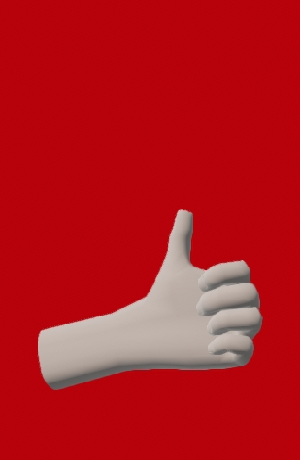
\includegraphics[width=\textwidth]{OK}
	\caption{Model: OK}
	\label{fig:modelOk}
	\end{subfigure}
	~
	\begin{subfigure}[b]{0.22\textwidth}
	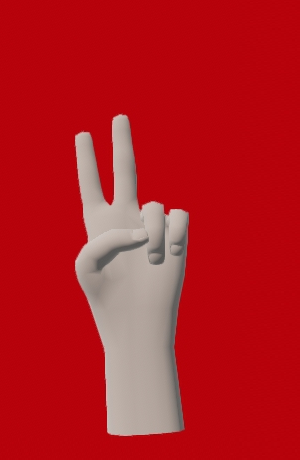
\includegraphics[width=\textwidth]{PEACE}
	\caption{Model: Pokój}
	\label{fig:modelPeace}
	\end{subfigure}
	~
	\begin{subfigure}[b]{0.22\textwidth}
	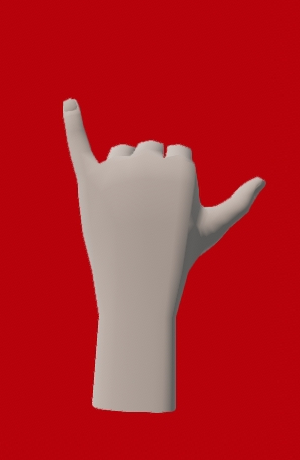
\includegraphics[width=\textwidth]{MAHALO}
	\caption{Model: Mahalo}
	\label{fig:modelMahalo}
	\end{subfigure}
	~
	\begin{subfigure}[b]{0.22\textwidth}
	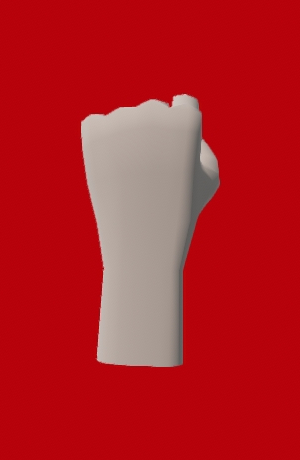
\includegraphics[width=\textwidth]{FIST}
	\caption{Model: Pięść}
	\label{fig:modelFist}
	\end{subfigure}
\caption{Modele animacji dłoni.}
\label{fig:modele}
\end{figure}
Tak jak powiedziano wcześniej, do importowania modeli używana jest wtyczka stworzona przez \textit{Google}. Jednak od tego etapu do wyświetlenia modelu na ekranie jest jeszcze kilka kroków które należy wykonać. Przede wszystkim nazwy modeli w aplikacji przechowywane są w tablicy typu \textit{String}. Niestety ten etap nie jest automatyczny, w związku z czym trzeba ręcznie podać nazwę modelu w aplikacji, aby był brany pod uwagę. Po wywołaniu funkcji \textit{renderView()}, zostaje wywołana funkcja \textit{assignModelNames()} której jedynym zadaniem jest przypisanie kolejnym pozycją w tablicy kolejnych nazw modeli z których chcemy korzystać. Nazwy te to pliki wygenerowane przez wtyczkę z rozszerzeniem \textit{.sfb}. Następnie wywoływana jest pętla w której dla każdej nie pustej nazwy w tablicy zostaje wywoływany wzorzec projektowy \textit{builder}, na klasie \textit{ModelRenderable}w celu stworzenia finałowej wersji modelu. Modele te po "zbudowaniu" wykorzystują klasie \textit{CompletableFuture<>} która pozwala wywołać metodę która zostanie wywołana na danym modelu gdy tylko ten zostanie ukończony. Metodą tą jest \textit{onRenderableLoades(ModelRenderable,String)} w której to modele kolejno są dodawane do zbioru przechowywanych modeli w aplikacji. Kod aplikacji~\ref{lst:loadScene} prezentuje omówione zagadnienia.
\begin{lstlisting}[caption={Generowanie sceny i modeli użytych w aplikacji.},captionpos=b,label={lst:loadScene},language = Java , frame = trBL , firstnumber = last , escapeinside={(*@}{@*)}]     
 	private void generateSceneView() {
        renderView();
        assignModelNames();

        for (String s : modelNames) {
            if (s != null && !s.equals("")) {
                ModelRenderable.builder()
                        .setSource(getContext(), Uri.parse(s))
                        .build()
                        .thenAccept(renderable -> onRenderableLoades(renderable,s))
                        .exceptionally(
                                throwable -> {
                                    Log.e("Model", "Unable to load Renderable.", throwable);
                                    return null;
                                });
            }
        }

        loadStartingModel();

        new Thread (this::startDataListener).start();
    }

    private void renderView() {
        sceneView = vw.findViewById(R.id.scene_view);
        [...]
        coreNode = new Node();
		[...]
        sceneView.getScene().addChild(coreNode);
    }                                             
\end{lstlisting}
Gdy omawiany proces zakończy się, zostaje wywołana funkcja \textit{loadStartingModel()} która jest odpowiedzialna za przygotowanie sceny, zanim dojdzie do połączenia z rękawicą kontrolerem. W funkcji tej zostaje wybrany model który zostaje przypisany do sceny jako pierwszy, a dzieję się to poprzez sprawdzanie w nowym wątku dziesięć razy na sekundę czy wybrany model został już wygenerowany przez wzorzec projektowy oraz czy został dodany do zbioru gotowych modeli. Gdy warunek ten zostanie spełniony wywoływana jest metoda \textit{setrenderable(Renderable)} która pozwala na przypisanie modelu do węzła już znajdującego się na scenie. Ostatnim elementem jest wywołanie nowego wątku w którym to ustawiany jest wysłuchiwacz zmian. Funkcja ta pokazana jest na listingu~\ref{lst:listener}. Sposób jej działanie polega na uruchomieniu nieskończonej pętli w której to są sprawdzane wartości flag zmiany danych. Flagi te są ustawiane jako prawdziwe w przypadku otrzymania nowych danych z kontrolera, co widać w ostatniej linii listingu~\ref{lst:setChar}. W ten oto sposób są sprawdzane flagi \textit{isCalibrating} co zostanie opisane w sekcji~\ref{subsec:kalibracja}, \textit{ismIsStateChanged()} dla zmian danych pochodzących z IMU z zagnieżdżonymi flagami \textit{renderRotation} oraz \textit{renderPosition}, sprawdzającymi czy użytkownik chce aby brano odpowiednio rotacji i pozycję pod uwagę podczas generowanie modelu. Działanie aplikacji w przypadku gdy te warunku są spełnione zostaną opisane odpowiednio w sekcjach~\ref{subsec:rotacja} oraz~\ref{subsec:przesuniecie}. Ostatnią flagą jest flaga pochodząca z klasy \textit{VrGlove} - \textit{ismIsFingersReadings()}, mówiąca czy dane z sensorów palców się zmieniły. 
\begin{lstlisting}[caption={Wysłuchiwacz zmian w danych rękawicy.},captionpos=b,label={lst:listener},language = Java , frame = trBL , firstnumber = last , escapeinside={(*@}{@*)}]     
private void startDataListener() {
        while(true){
            if(!isCalibrating){
                if(VrGlove.ismIsStateChanged()){
                   if(renderRotation){
                       [...]
                    }

                    if(renderPosition){
                        [...]
                }
                
                if(VrGlove.ismIsFingersReadings()){
                    [...]
                }
            }
        }
    }                                            
\end{lstlisting}
	
	\subsection{Rozpoznanie i animacja modelu}
	\label{subsec:rozpoznanie}
	Jeżeli dane się zmieniły od ostatniego wywołania tej funkcji wartość \\  \textit{VrGlove.ismIsFingersReadings()} zwróci prawdę co oznacza że wykona się kod rozpoznania i ewentualnej zmiany modelu. Kod ten jest obsługiwany poprzez wywołanie funkcji \textit{replaceModel()} i nie zależnie od jej działania, zawsze po jej zakończeniu wywoływana jest linia kodu \textit{VrGlove.setmIsFingersReadings(false);}, dzięki której uzyskano pewność że ten sam zestaw danych nie będzie rozpatrywany wielokrotnie -  flaga ta zostanie zmieniona na prawdziwą dopiero gdy nowe dane trafią do aplikacji. Najważniejsze kroki funkcji \textit{replaceModel()} zostaną opisane poniżej. \\
	Powiedziano wcześniej że w celu dodania nowego modelu potrzebna jest jego model, który następnie jest importowany przez plugin a nazwa zostaje dodane do tablicy w której przechowywane są nazwy modeli z rozszerzeniem \textit{.sfb}. Rzeczywiście dzięki temu model znajduję się w ramach aplikacji jednak z perspektywy użytkownika nigdy nie zostanie on zaobserwowany. Dzieję się tak z powodu ostatniego elementu który należy dodać w celu dodania nowego modelu - dla odpowiadającej mu pozycji w tablicy należy dodać tablicę pięciu liczb -1/0/1. Tablica ta odpowiednio reprezentuje pozycje palców na modelu który jest dodawany, gdzie 0 oznacza palec zgięty, 1 palec wyprostowany natomiast -1 pozycję pomiędzy tymi wygięciami. Z powodów opisanych w rozdziale~\ref{ch:rozwoj} nie zaleca się stosowania wartości -1. W ten oto sposób możemy rozpatrzeć nowe dane w kontekście istniejących modeli. \\
	W aplikacji zostały zdefiniowane wartości minimalne oraz maksymalne dla każdego sensorów. Wartości te zostały zczytane dla każdego palca gdy wszystkie palce były wyprostowane, a także gdy każdy z palców po kolei był zginany tak bardzo jak to było możliwe. Wartości te zostały pobrane eliminując wartości skrajne, czekając aż odczyty z palców się unormują wokół pewnego zakresu. W trakcie porównywania jest brany pod uwagę margines błędu rzędu $\pm 30$ wiec są to jedynie przybliżone wartości. Rezultaty tych wartości prezentuje tabela poniżej:
\begin{center}
\begin{tabular}{|c|c|c|}
\hline
Palec & Minimalna wartość & Maksymalna wartość \\ \hline
Kciuk & 520 & 680\\ \hline
Wskazujący & 400 & 580\\ \hline
Środkowy & 520 & 670\\ \hline
Serdeczny & 500 & 750 \\ \hline
Mały & 480 & 620 \\ \hline
\hline
\end{tabular}
\end{center}
Mając do dyspozycji pokazane dane, pierwszych etapem analizy sensorów palców jest sprawdzenie jak odnoszą się ona względem tych danych. Dla każdego palca następuje porównanie do wartości minimalnej oraz maksymalnej. Jeżeli wartość sensora odpowiada wartości minimalnej $\pm 30$ zostaje przypisane dla tego palca 0, w przypadku wartości maksymalnej 1 a w pozostałych przypadkach -1. Mając do dyspozycji wartości w jakiej znajduje się obecnie dłoń, oraz wymagania położenia każdego z palców w danym modelu, dokonano porównania tych stanów. Jeżeli rozpoznano model, i model ten nie jest obecnie prezentowanym modelem - funkcja zwraca nowy model który należy wygenerować. Opisany proces pokazuje listing~\ref{lst:recognize}.
\begin{lstlisting}[caption={Rozpoznianie danych sensorów i wzoru modelu.},captionpos=b,label={lst:recognize},language = Java , frame = trBL , firstnumber = last , escapeinside={(*@}{@*)}]     
for (int i =0; i < fingersReadings.length; i++){
            if(fingersReadings[i] < sensorsBoundarySettings[i][0]+30.0f){
                pattern[i] = 0;
            }else if(fingersReadings[i] > sensorsBoundarySettings[i][1]-30.0f){
                pattern[i] = 1;
            }else{
                pattern[i] = -1;
            }
        }   
        for(int[] i : modelRequirements){
            for (int j = 0; j < i.length; j++){
                if(i[j] != pattern[j]){
                    break;
                }
                m = models[j];
            }
            if(m != null){
                break;
            }
        }
        if (m != null){
            if(m != currentModel){
                return m;
            }
        }
        return null;                                                        
\end{lstlisting}	
Generowanie nowego modelu odbywa się poprzez wywołanie funkcji \textit{assignModelToNode(ModelRenderable)}, rozpoczynając od sprawdzenia czy przekazany model posiada wartość a następnie wywołuję sekwencje zadań na wątku interfejsu. Tak jak powiedziano wcześniej model jest wyświetlany na scenie poprzez połączenie go z węzłem. Jednak aby uniknąć powtarzania tych samych sekwencji oraz zachować płynność obrazu pomiędzy głównym węzłem a modelem został dodany węzeł pośredni. Główny węzeł-rodzic odpowiada za położenie na ekranie a także rotację względem punktu początkowego. Węzeł-dziecko natomiast jest zmieniany w zależności od modelu który należy zaprezentować na ekranie. Sekwencja uruchamiana w interfejsie rozpoczyna się od utworzenia nowego węzła i przypisania mu nowego modelu, który został wybrany do prezentacji użytkownikowi. Następnie dochodzi do usunięcia obecnego modelu poprzez usunięcie ze ze sceny węzła z który model ten był powiązany a następnie dodanie węzła z nowym modelem. Cały ten proces pokazuje listing~\ref{lst:swap}, jednocześnie podsumowując proces obsługi modeli w projekcie.
\begin{lstlisting}[caption={Zamiana węzłów z powiązanymi modelami w interfejsie użytkownika.}, captionpos=b,label={lst:swap},language = Java , frame = trBL , firstnumber = last , escapeinside={(*@}{@*)}]     
Objects.requireNonNull(getActivity()).runOnUiThread(() ->{
                    Node render = new Node();
                    render.setRenderable(modelRenderable);
                    coreNode.removeChild(renderedNow);
                    renderedNow = render;
                    coreNode.addChild(render);
                    replacingInProgress = false;
        } );                                                      
\end{lstlisting}

	\subsection{Rotacja}
	\label{subsec:rotacja}
	W sekcji~\ref{subsec:rozpoznanie} pokazano w jaki sposób umiejscowiono główny węzeł na scenie prezentowanej użytkownikowi, a także w jaki sposób modele są przypisywane do węzłów pomocniczych. Tak jak wspomniano, aby model mógł się poruszać dokonywane są zmiany na węźle głównym, które jako efekt końcowy dotyczą również węzłów pomocniczych, czyli z perspektywy użytkownika - modelu dłoni. W pierwszej kolejności zostanie pokazane jak dane z IMU zostają zamienione na rotację modelu. Aby rotacja była brana pod uwagę przede wszystkim w interfejsie użytkownika przycisk typu przełącznik musi być w pozycji włączonej - oznacza to że flaga \textit{renderRotation} jest prawdziwa i aplikacja będzie dokonywała obliczeń. W tym celu wykorzystywane są dane zarówno z żyroskopu jak i akcelerometru. W pierwszej kolejności wywoływana jest funkcja \textit{calculateRotation()}, która pobiera aktualnie dostępne dane i o ile dane istnieją dla obu sensorów, zostają wywołane funkcje \textit{calculateAccAngles} oraz \textit{calculateGyroAngles}. Pierwsza z nich odpowiedzialna jest za wyliczenie kątów kontrolera na podstawie akcelerometru. W przypadku akcelerometru dla odczytów X,Y,Z, kąty te mogą zostać wyliczone dla przechyłu bocznego (ang. roll) oraz nachylenia (ang. pitch), przy użyciu następujących wzorów 
	$$
		Roll = \arctan\left(\frac{Y}{\sqrt{X^2 + Z^2}}\right)
	$$$$
		Pitch = \arctan\left(\frac{-1 * X}{\sqrt{Y^2 + Z^2}}\right)
	$$
W ten sposób otrzymujemy wartości kątów w radianach. Aby uzyskać kąty w stopniach należy wynik przemnożyć przez \begin{Large}$\frac{180}{\pi}$\end{Large}. W ten oto sposób otrzymane kąty z akcelerometru trafiają do funkcji \textit{normalizeAngles}, która upewnia się że kąt zwracany przez \textit{Roll} nie przekroczy $\pm 85$ stopni, aby uniknąć blokady gimbala, a także w przypadku ciągłej rotacji, gdy kontroler wykona pełen obrót, czyli $360^o$, stopnie te wracają do pozycji początkowej czyli $0^o$. W ten oto sposób otrzymujemy końcowy efekt dla akcelerometru i wykonuję się funkcja obliczania kątów z danych żyroskopu. Jak stwierdzono w dziale~\ref{sec:oprogramowanie}, zadaniem żyroskopu w tym projekcie jest jedynie wyliczanie kątów, w związku z czym dane żyroskopy zostały zamienione na stopnie już po stronie kontrolera. Oznacza to że funkcja \textit{calculateGyroAngles} jedynie dodaje do aktualnego stanu kątów urządzenia, które w stanie początkowym wynoszą zero, nowo przesłane wyniki z żyroskopu. Kąty te następnie są normowane tak jak w przypadku akcelerometru. Końcową częścią obliczania kątów urządzenia jest zastosowanie filtra komplementarnego na podstawie obliczonych kątów z sensorów. Filtr komplementarny służy jako mechanizm kontrolowania błędu odchylenia gromadzonego przez żyroskop w długim okresie czasu, poprzez zastosowania małej korekty z bardziej dokładnego lecz wolniejszego akcelerometru. W celu skorygowania skrętu (ang. Yaw) używa się magnetometru, jednak w tym projekcie nie wykorzystano tego sensora w związku z czym jedynie dane z żyroskopu są brane pod uwagę. Poprzez ustawienie parametru filtra, można zmienić stopień w jakim akcelerometr koryguje dane - w aplikacji filtr jest ustawiony na $94\%$, co oznacza że akcelerometr koryguje dane w $6\%$. Implementacja filtra jest pokazana na listingu~\ref{lst:compFiltr}~\cite{gimbal}.
\begin{lstlisting}[caption={Implementacja filtru komplementarnego.}, captionpos=b,label={lst:compFiltr},language = Java , frame = trBL , firstnumber = last , escapeinside={(*@}{@*)}]     
float filterValue = 0.94f;
result[0] = filterValue * gyroAngles[0] + (1 - filterValue) * tmp[0];
result[1] = filterValue * gyroAngles[1] + (1 - filterValue) * tmp[1];
result[2] = gyroAngles[2];                                                    
\end{lstlisting}
W ten sposób kończy się obliczanie rotacji kontrolera według każdej z osi. Zostaje one dopasowana do orientacji dłoni na ekranie poprzez wykorzystanie zamiany kątów podanych w stopniach na kwaternion z wykorzystaniem metody \textit{axisAngle(Vector3,float)}, a następnie w celu określenia rotacji końcowej przemnożenie przez siebie poszczególnych rotacji. W mnożeniu tym ważna jest kolejność wykonywania, dlatego też jako element środkowy musi wystąpić kąt określony według osi X, który został zablokowany w przedziale $\pm 85^o$, co nie pozwala na powstanie blokady gimbala. Wynik mnożenia poszczególnych rotacji jest obrotem który należy wykonać, poprzez funkcję \textit{setLocalRotation(Quaternion)}. W ten oto sposób aplikacja obsługuję rotację modelu. Proces ten pokazuje listing~\ref{lst:kwat}.
\begin{lstlisting}[caption={Obrót węzła na podstawie obliczonych kątów.}, captionpos=b,label={lst:kwat},language = Java , frame = trBL , firstnumber = last , escapeinside={(*@}{@*)}]     
Quaternion[] quat = new Quaternion[3];
calculateRotation();
quat[0] = Quaternion.axisAngle(new Vector3(0.0f,0.0f,-1.0f),modelAngles[0]); 
quat[1] = Quaternion.axisAngle(new Vector3(1.0f,0.0f,0.0f),modelAngles[1]);
quat[2] = Quaternion.axisAngle(new Vector3(0.0f,1.0f,0.0f),modelAngles[2]);
Quaternion resultOrientation = Quaternion.multiply(Quaternion.multiply(quat[1],quat[0]),quat[2]);
this.coreNode.setLocalRotation(resultOrientation);
\end{lstlisting}
	
	\subsection{Przesunięcie}
	\label{subsec:przesuniecie}	
	Ostatnim elementem zmieniającym model jest ustalenie zmiany w jego położeniu, tak aby móc odwzorować ten sam ruch na ekranie. Opcja ta gdy jest włączona, ustawia flagę \textit{renderPosition} na prawdziwą pozwalając na obliczanie pozycji. W prezentowanej aplikacji, do tego celu wykorzystywany jest tylko jedne sensor - akcelerometr. Na podstawie tych danych wylicza pozycję kontrolera funkcja \textit{parseAccDataToDisplacement()}, a następnie podobnie jak w przypadku rotacji, na głównym węźle wywoływana jest funkcja która ustawia nową pozycję. Funkcja ta to \textit{setLocalPosition(Vecotr3)}. Aby osiągnąć pozycję kontrolera na podstawie danych z akcelerometru, które są podawane w \begin{Large}
	$\frac{m}{s^2}$
	\end{Large}, należy wykonać podwójne całkowanie. Dzięki temu najpierw osiągniemy prędkość w {\Large$\frac{m}{s}$}, a następnie wartość w $m$. W tym celu podczas otrzymania nowych danych zapisywany jest czas w którym te dane pozyskano, i tak jak w przypadku danych z żyroskopu, dane te są mnożone przez upływ czasu pomiędzy pomiarami. Oczywiście wyniki z akcelerometru podlegają działaniu grawitacji, w związku z czym nie jest to jedynie prędkość poruszania się kontrolera. Wektor grawitacji jest pozyskiwany w trakcie kalibracji urządzenia co będzie opisana w sekcji~\ref{subsec:kalibracja}. Oprócz tego w prezentowanym projekcie mamy do czynienia z kontrolerem który zmienia swoją rotację, co oznacza że również wektor grawitacji zmienia się w zależności od orientacji w przestrzeni względem układu orientacji ziemi. W związku z tym aby osiągnąć prawidłowe pomiary przed całkowaniem danych, należy przywrócić pozyskane dane z orientacji w której się aktualnie znajdują, do orientacji początkowej, usunąć wektor grawitacji który w takiej pozycji pozyskano a następnie przywrócić orientację urządzenia. Dzięki temu dane które zostaną podwójnie scałkowane zwrócą wynik samego przemieszczenia bez dodatkowych sił oddziałujących na akcelerometr. W aplikacji proces ten jest osiągnięty poprzez stworzenie macierzy rotacji na podstawie obecnej orientacji modelu, dzięki której przemnożono wektor danych pozyskany z akcelerometru. Od wektora wynikowego została odjęta przechowywana grawitacja pozyskana przy kalibracji, a następnie wektor został przemnożony przez odwróconą macierz rotacji, dzięki czemu przywrócono oryginalną rotację. W ten sposób dane zostały scałkowane uzyskując pozycję. Omawiane metody prezentuje listing~\ref{lst:pos}~\cite{displacement3}~\cite{displacement2}~\cite{displacement}.
	\begin{lstlisting}[caption={Listing obrazujący obliczanie przemieszczenia kontrolera.}, captionpos=b,label={lst:pos},language = Java , frame = trBL , firstnumber = last , escapeinside={(*@}{@*)}]  
final float dT = (currentTime - lastTimestamp) * dtNanoToSec;
[...]	   
float[] rotationM = getRotationMatrixFromAngles(tmpAngles);
[...]
float[] accDataPostRotation = removeRotation(accSet, rotationM);
for (int i = 0; i<accDataPostRotation.length; i++ ){
	accDataPostRotation[i] -= gravityV[i];
    }
float[] invMatrix = invertMatrix(rotationM);
[...]
accDataWithoutG = multiplyMatrix3xVector(invMatrix, accDataPostRotation );
[...]
for(int i = 0; i < velocity.length; i++){
	velocity[i] += accDataWithoutG[i]*dT;
	pos[i] += velocity[i]*dT;
}
[...]
lastTimestamp = currentTime;
\end{lstlisting}
	
	\subsection{Kalibracja}
	\label{subsec:kalibracja}
	Do tej pory zostały opisane elementy sterujące animacją modelu, jego pozycją oraz orientacją, a także flagi pozwalające na wyłączenie orientacji oraz położenia. Ostatnim elementem odpowiedzialnym za zmiany na ekranie jest kalibracja modelu z kontrolerem. Dzieje się to poprzez wciśnięcie przycisku FAB na ekranie. Zmienia on wartość flagi \textit{isCalibrating}, nie pozwalając tym samym na wykonywania nowych akcji na modelu dłoni. Oprócz tego kalibracja jest wykonywana gdy nawiązano połączenie z kontrolerem oraz gdy użytkownik zmieni pozycję przycisków przełączników odpowiedzialnych za orientację i położenie. W wysłuchiwaczu przycisku FAB oprócz zatrzymania zmian na obecnie działającym modelu, resetują się wszystkie zmienne jakie do tej pory zostały pozyskane. Oznacza to że kąty modelu znów ustawione są jako zero wokół każdej osi, zmiana położenie jest liczona od nowa, ustawiony zostaje ponownie model początkowy a także jego pozycja i orientacja zostaje przywrócona do pozycji początkowej. Aby dać na dostosowanie się do tych zmian użytkownikowi, aplikacja wyświetla nowy model po upływie trzech sekund, ciągle wyświetlając przy tym wiadomość na ekranie informując użytkownika ile czasu mu się pozostało. Podczas kalibracji oczekuje się od użytkownika ustawienia lewej dłoni z wyprostowanymi palcami w taki sposób aby kciuk wskazywał ciało użytkownika a także aby utrzymać tą pozycję bez dodatkowych ruchów. Pozycja ta jest pozycją początkową modelu i to użytkownik musi się do niej zastosować. Gdy tylko kalibracja jest zakończona, pierwszym etapem przed wznowieniem pracy na ekranie jest pobranie aktualnej wartości akcelerometru - wartość ta jest pobierana przy założeniu że użytkownik nie wykonuje żadnych dodatkowych ruchów i jest zapisywana jako wektor grawitacji oddziałujący na model w pozycji kalibracyjnej. W tym momencie pozycja w jakiej się znajduje rękawica-kontrolera, jest uznawana za pozycję wyjściową, od której będą mierzone kąty obrotów wokół osi a także przemieszczenie, a modele będą się zmieniać w zależności od danych z sensorów na palcach. W ten oto sposób zaprezentowano wszystkie elementy i zasady działania aplikacji wykorzystującej do działania dane z rękawicy-kontrolera.
	
	

